\documentclass[10pt]{article}

\usepackage[margin=0.75in]{geometry}
\usepackage{amsmath,amsthm,amssymb}
\usepackage{xcolor}
\usepackage{cancel}
\usepackage{graphicx}
\usepackage{changepage}
\usepackage{circuitikz}
\usepackage{pgfplots}
\usepackage{physics}
\usepackage{hyperref}
\usepackage{siunitx}
\usepackage{fontspec}
\usepackage{relsize}
\usepackage{subfig}
\usepackage{todonotes}
\usepackage{multicol, multirow, booktabs}
\usepackage[breakable]{tcolorbox}
\usepackage[inline]{enumitem}

\theoremstyle{definition}
\newtheorem{problem}{Problem}
\newtheorem{soln}{Solution}

\pgfplotsset{compat=newest}
\usetikzlibrary{lindenmayersystems}
\usetikzlibrary{arrows}
\usetikzlibrary{calc}
\usetikzlibrary{positioning, fit}
\usetikzlibrary{3d, perspective}

\definecolor{incolor}{HTML}{303F9F}
\definecolor{outcolor}{HTML}{D84315}
\definecolor{cellborder}{HTML}{CFCFCF}
\definecolor{cellbackground}{HTML}{F7F7F7}
\newcommand{\ui}{\hat{i}}
\newcommand{\uj}{\hat{j}}
\newcommand{\uk}{\hat{k}}
\newcommand{\ux}{\hat{\mathbf{x}}}
\newcommand{\uy}{\hat{\mathbf{y}}}
\newcommand{\uz}{\hat{\mathbf{z}}}
\newcommand{\primed}[1]{{#1^\prime}}
\pgfdeclarelayer{background}  
\pgfsetlayers{background,main}
\AtBeginDocument{\RenewCommandCopy\qty\SI}

\makeatletter
\newcommand{\boxspacing}{\kern\kvtcb@left@rule\kern\kvtcb@boxsep}
\makeatother
\newcommand{\prompt}[4]{
    \ttfamily\llap{{\color{#2}[#3]:\hspace{3pt}#4}}\vspace{-\baselineskip}
}

\newcommand{\thevenin}[2]{
  \begin{center}
    \begin{circuitikz} \draw
      (0,0) -- (2,0) to[battery1, l_=$V_{Th}\eq#1$] (2,2) 
      to[resistor, l_=$R_{Th}\eq#2$] (0,2)
      ;
      \draw [o-] (-.07,2.079);
      \draw [o-] (-.07,0.079);
    \end{circuitikz}
  \end{center}
}

\newcommand{\norton}[2]{
  \begin{center}
    \begin{circuitikz} \draw
      (0,0) -- (3,0) to[american current source, l_=$I_{N}\eq#1$] (3,2) -- (0,2) (2,0)
      to[resistor, l=$R_{N}\eq#2$] (2,2)
      ;
      \draw [o-] (-.07,2.079);
      \draw [o-] (-.07,0.079);
    \end{circuitikz}
  \end{center}
}

\DeclareMathOperator{\Div}{div}
\DeclareMathOperator{\Curl}{curl}

\newcommand{\highlight}[1]{\colorbox{yellow}{$\displaystyle #1$}}

\newcommand{\ti}[1]{\widetilde{#1}}

\newfontface{\Kaufmann}{Kaufmann}
\DeclareTextFontCommand{\kf}{\Kaufmann}
\newcommand{\scriptr}{\fontsize{12pt}{12pt}\kf{r}}

\newfontface{\KaufmannB}{Kaufmann Bd BT}
\DeclareTextFontCommand{\kfb}{\KaufmannB}
\newcommand{\bscriptr}{\fontsize{12pt}{12pt}\kfb{r}}
\newcommand{\justif}[2]{&{#1}&\text{#2}}
\newcommand{\bv}[1]{\mathbf{#1}}

\title{Physics 3200Y: Assignment I}
\author{Jeremy Favro (0805980) \\ Trent University, Peterborough, ON, Canada}
\date{\today}

\begin{document}
\maketitle

% PROBLEM 1
\begin{problem}
A hollow cone has a constant surface charge density $\sigma$. The cone's vertex is at $z = 0$ and its axis lies along the
positive $z$-axis. It has a height $h$, which is also the radius of the cone at its widest end (the top). You are asked
to find the potential difference $V (h) - V (0$) between the top (on the cone's axis) and the vertex.
\begin{enumerate}[label=(\alph*)]
  \item Draw a picture that defines $\bv{r}$, $\primed{\bv{r}}$, $\scriptr$, etc.
  \item Discuss how you will parameterize your surface and find expressions for $\primed{\bv{r}}$ and $d\primed{a}$ in terms of your parameters.
  \item Write out and solve the integrals for $V (h)$ and $V (0)$ to find the final answer. The integral for $V (0)$ is easy
        to do, and I have some hints for the integrals for $V (h)$. First, I found it helpful to make the substitution
        $\primed{z}=h/2+t$, and then with a little bit of work the integral simplifies to a constant times something of the
        form
        $$\int_{-a}^{a}\frac{dt}{\sqrt{a^2+t^2}}=2\sinh^{-1}(\frac{1}{\sqrt{2}})$$
        Show your work. Don't simply look up the integral!
\end{enumerate}
\end{problem}
\begin{soln}~
  \begin{enumerate}[label=(\alph*)]
    \item \newpage
    \item I will parametrize the cone in spherical coordinates in terms of $\primed{\theta}$, $\primed{\phi}$ and $\primed{r}$.
          Here though $\theta$ is fixed so our usual mapping to spherical becomes
          \begin{align*}
            \primed{x} & =\primed{r} \sin \left(\pi/4\right)\cos\primed{\phi}=\primed{r}\cos\primed{\phi}/\sqrt{2} \\
            \primed{y} & =\primed{r} \sin \left(\pi/4\right)\sin\primed{\phi}=\primed{r}\sin\primed{\phi}/\sqrt{2} \\
            \primed{z} & =\primed{r} \cos \left(\psi/4\right)=\primed{r}/\sqrt{2}
          \end{align*}
          for
          $$\primed{\bv{r}}=\primed{x}\ux+\primed{y}\uy+\primed{z}\uz.$$
          Our area element becomes
          $$d\primed{a}=\primed{r}\sin\left(\pi/4\right)d\primed{r}d\primed{\phi}=\primed{r}d\primed{r}d\primed{\phi}/\sqrt{2}.$$
          This means that we're going to be sweeping out the area rotating around $z$ and increasing $\primed{r}$. The obvious bounds
          then for the $\primed{\phi}$ integral are $0\leq \primed{\phi}\leq 2\pi$ but for
          $\primed{r}$ we want to sweep from zero radius out to the tip of the cone. Because the cone forms a right triangle
          with sides of length $h$ the maximum point will be at, by pythagorean theorem,
          $$\sqrt{h^2+h^2}=\sqrt{2}h$$
    \item Setting up a few things first we have
          $$\scriptr=\abs{\bv{r}-\primed{\bv{r}}}
            =\sqrt{\left(x-\primed{r}\cos\primed{\phi}/\sqrt{2}\right)^2
              +\left(y-\primed{r}\sin\primed{\phi}/\sqrt{2}\right)^2
              +\left(z-\primed{r}/\sqrt{2}\right)
            }.
          $$
          Now using
          $$V(\bv{r})=\frac{1}{4\pi\epsilon_0}\int_{S}\frac{\sigma(\primed{r})}{\scriptr}\,d\primed{a}$$
          which in our case becomes
          $$V(\bv{r})=\frac{\sigma}{4\pi\epsilon_0}
            \int_{0}^{2\pi}\int_{0}^{\sqrt{2}h}
            \frac{1}{\sqrt{\left(x-\primed{r}\cos\primed{\phi}/\sqrt{2}\right)^2
                +\left(y-\primed{r}\sin\primed{\phi}/\sqrt{2}\right)^2
                +\left(z-\primed{r}/\sqrt{2}\right)
              }}
            \,\primed{r}d\primed{r}d\primed{\phi}/\sqrt{2}$$
          Now,
          \begin{enumerate}[label=(\roman*)]
            \item Our integral for $V(0,0,0)$ simplifies greatly,
                  \begin{align*}
                    V(0) & =\frac{\sigma}{4\sqrt{2}\pi\epsilon_0}
                    \int_{0}^{2\pi}\int_{0}^{\sqrt{2}h}
                    \frac{\primed{r}}{\sqrt{\left(0-\primed{r}\cos\primed{\phi}/\sqrt{2}\right)^2
                        +\left(0-\primed{r}\sin\primed{\phi}/\sqrt{2}\right)^2
                        +\left(0-\primed{r}/\sqrt{2}\right)^2
                      }}
                    \,d\primed{r}d\primed{\phi}                   \\
                         & =\frac{\sigma}{4\sqrt{2}\pi\epsilon_0}
                    \int_{0}^{2\pi}\int_{0}^{\sqrt{2}h}
                    \frac{\primed{r}}{\sqrt{
                    {\primed{r}}^2\cos^2\primed{\phi}/2
                    +{\primed{r}}^2\sin^2\primed{\phi}/2
                    +{\primed{r}}^2/2
                    }}
                    \,d\primed{r}d\primed{\phi}                   \\
                         & =\frac{\sigma}{4\pi\epsilon_0}
                    \int_{0}^{2\pi}\int_{0}^{\sqrt{2}h}
                    \frac{\primed{r}}{\sqrt{
                    {\primed{r}}^2
                    +{\primed{r}}^2
                    }}
                    \,d\primed{r}d\primed{\phi}                   \\
                         & =\frac{\sigma}{2\epsilon_0}
                    \int_{0}^{\sqrt{2}h}
                    \frac{\primed{r}}{\sqrt{
                        2{\primed{r}}^2
                      }}
                    \,d\primed{r}                                 \\
                         & =\frac{\sigma}{2\sqrt{2}\epsilon_0}
                    \int_{0}^{\sqrt{2}h}
                    \,d\primed{r}=\frac{\sigma h}{2\epsilon_0}
                  \end{align*}
            \item Now our integral for $V(0,0,h)$,
                  \begin{align*}
                    V(0,0,h) & =\frac{\sigma}{4\sqrt{2}\pi\epsilon_0}
                    \int_{0}^{2\pi}\int_{0}^{\sqrt{2}h}
                    \frac{\primed{r}}{\sqrt{\left(0-\primed{r}\cos\primed{\phi}/\sqrt{2}\right)^2
                        +\left(0-\primed{r}\sin\primed{\phi}/\sqrt{2}\right)^2
                        +\left(h-\primed{r}/\sqrt{2}\right)^2
                      }}
                    \,d\primed{r}d\primed{\phi}                                          \\
                             & =\frac{\sigma}{4\sqrt{2}\pi\epsilon_0}
                    \int_{0}^{2\pi}\int_{0}^{\sqrt{2}h}
                    \frac{\primed{r}}{\sqrt{{\primed{r}}^2\cos^2\primed{\phi}/2
                    +{\primed{r}}^2\sin^2\primed{\phi}/2
                    +\left(h-\primed{r}/\sqrt{2}\right)^2
                    }}
                    \,d\primed{r}d\primed{\phi}                                          \\
                             & =\frac{\sigma}{4\sqrt{2}\pi\epsilon_0}
                    \int_{0}^{2\pi}\int_{0}^{\sqrt{2}h}
                    \frac{\primed{r}}{\sqrt{
                        {\primed{r}}^2/2
                        +\left(h-\primed{r}/\sqrt{2}\right)^2
                      }}
                    \,d\primed{r}d\primed{\phi}                                          \\
                             & =\frac{\sigma}{4\sqrt{2}\pi\epsilon_0}
                    \int_{0}^{2\pi}\int_{0}^{\sqrt{2}h}
                    \frac{\primed{r}}{\sqrt{
                        {\primed{r}}^2/2
                        +h^2-2h\primed{r}/\sqrt{2}+\primed{r}^2/2
                      }}
                    \,d\primed{r}d\primed{\phi}                                          \\
                             & =\frac{\sigma}{2\sqrt{2}\epsilon_0}
                    \int_{0}^{\sqrt{2}h}
                    \frac{\primed{r}}{\sqrt{
                        (x-h/\sqrt{2})^2+h^2/2
                      }}
                    \,d\primed{r}                                                        \\
                             & =\frac{\sigma}{2\sqrt{2}\epsilon_0}
                    \int_{0}^{\sqrt{2}h}
                    \frac{u+h/\sqrt{2}}{\sqrt{
                        u^2+h^2/2
                      }}
                    \,du\quad\rightsquigarrow\quad u=\primed{r}-h/\sqrt{2}\implies dx=du \\
                             & =\frac{\sigma}{2\sqrt{2}\epsilon_0}
                    \left[\int_{0}^{\sqrt{2}h}
                    \frac{u}{\sqrt{
                        u^2+h^2/2
                      }}
                    \,du+h/\sqrt{2}\int_{0}^{\sqrt{2}h}
                    \frac{1}{\sqrt{
                        u^2+h^2/2
                      }}
                    \,du\right]                                                          \\
                  \end{align*}
                  Which I'll solve separately,
                  \begin{align*}
                     & =\int_{0}^{\sqrt{2}h}
                    \frac{u}{\sqrt{
                        u^2+h^2/2
                      }}
                    \,du                                                                                                                                                 \\
                     & =\frac{1}{2}\int_{0}^{\sqrt{2}h}
                    \frac{1}{\sqrt{
                        v
                      }}
                    \,du\justif{\quad}{$v=u^2+h^2/2\implies dv=2udu$}                                                                                                    \\
                     & =\eval{\sqrt{v}}_{0}^{\sqrt{2}h}=\eval{\sqrt{u^2+h^2/2}}_{0}^{\sqrt{2}h}=\eval{\sqrt{\left(\primed{r}-h/\sqrt{2}\right)^2+h^2/2}}_{0}^{\sqrt{2}h} \\
                     & =\sqrt{\left(\sqrt{2}h-h/\sqrt{2}\right)^2+h^2/2}-\sqrt{\left(-h/\sqrt{2}\right)^2+h^2/2}                                                         \\
                     & =h-h                                                                                                                                              \\
                     & =0                                                                                                                                                \\
                  \end{align*}
                  And the other one:
                  \begin{align*}
                     & =h/\sqrt{2}\int_{0}^{\sqrt{2}h}
                    \frac{1}{\sqrt{
                        u^2+h^2/2
                      }}
                    \,du                                                                                                                                                                      \\
                     & =\sqrt{2}/h\int_{0}^{\sqrt{2}h}
                    \sec\alpha
                    \,d\alpha\justif{\quad}{$u=h/\sqrt{2}\tan\alpha\implies du=h/\sqrt{2}\sec^2\alpha d\alpha$}                                                                               \\
                     & =\sqrt{2}/h\eval{\ln\abs{\sec\alpha+\tan\alpha}}_{0}^{\sqrt{2}h}                                                                                                       \\
                     & =\sqrt{2}/h\eval{\ln\abs{\sqrt{1+\frac{2}{h^2}u^2}+\frac{\sqrt{2}}{h}u}}_{0}^{\sqrt{2}h}                                                                               \\
                     & =\sqrt{2}/h\eval{\ln\abs{\sqrt{1+\frac{2}{h^2}\left(\primed{r}-h/\sqrt{2}\right)^2}+\frac{\sqrt{2}}{h}\left(\primed{r}-h/\sqrt{2}\right)}}_{0}^{\sqrt{2}h}             \\
                     & =\eval{\ln\left(\left|h\sqrt{2{(\primed{r}-h/\sqrt{2})}^{2}+{h}^{2}}+\sqrt{2}h(\primed{r}-h/\sqrt{2})\right|\right)-2\ln\left(h\right)}_{0}^{\sqrt{2}h} \\
                     & =\sqrt{2}\ln\left(\sqrt{2}+1\right)h
                  \end{align*}
          \end{enumerate}
  \end{enumerate}
\end{soln}

% PROBLEM 2
\begin{problem}
Consider the infamous triple-plate capacitor (I just made that up), consisting of three parallel plates. Let the
middle plate lie in the xy plane, let the top plate lie a distance $d_1$ above it and the bottom plate lie a distance
$d_2$ below it. Assume that the capacitor charges in such a way that the top plate has a 2D charge density $\sigma$,
while the other two plates have charge densities $-\sigma/2$; treat the plates as infinite.
\begin{enumerate}[label=(\alph*)]
  \item Find the electric field everywhere along the $z$-axis, and the voltage differences between the different plates.
  \item Find the energy per unit area required to charge up the system by incrementally moving amounts of
        charge dQ from the lower two plates to the upper plate and calculating the work done for each increment.
        Describe carefully the sequence of steps in each case, since that is what you are being graded on.
  \item Show that you get the same answer for the work by integrating the electric field over all space.
\end{enumerate}
\end{problem}
\begin{soln}~
  \begin{enumerate}[label=(\alph*)]
    \item Here we can use superposition to find the electric field in the four regions of interest shown below,
          \begin{center}
            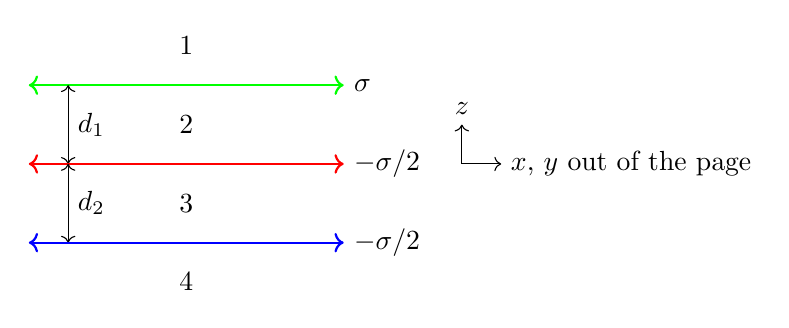
\begin{tikzpicture}
              \node at (2, 1.5) {$1$};
              \node at (2, 0.5) {$2$};
              \node at (2, -0.5) {$3$};
              \node at (2, -1.5) {$4$};

              \draw[<->, green, thick] (0,1) -- (4,1) node[black, right]{$\sigma$};
              \draw[<->, black] (0.5, 1) -- (0.5,0) node[midway, right]{$d_1$};
              \draw[<->, red, thick] (0,0) -- (4,0) node[black, right]{$-\sigma/2$};
              \draw[<->, black] (0.5, 0) -- (0.5,-1) node[midway, right]{$d_2$};
              \draw[<->, blue, thick] (0,-1) -- (4,-1) node[black,right]{$-\sigma/2$};

              \draw[->, black] (5.5, 0) -- (6,0) node[right]{$x$, $y$ out of the page};
              \draw[->, black] (5.5, 0) -- (5.5,0.5) node[above]{$z$};
            \end{tikzpicture}
          \end{center}
          By Gauss' law we have
          $$\int_S\bv{E}\cdot d\bv{a}=Q_{enc}/\epsilon_0.$$
          Here $Q_{enc}$ in terms of the given charge distribution is the charge per unit area ($\sigma$) times
          the area of the entire surface which we'll call $A$. This gets us
          $$\int_S \bv{E}\cdot d\bv{a}=\sigma A/\epsilon_0.$$
          Since the capacitor plates are infinite we can say that $\bv{E}=E_z\uz$ and we know that the area
          element for the $xy$ plane is $dxdy\uz$. This makes our integral
          $$\int\int \abs{E_z} dxdy=\abs{E_z}\int\int dxdy=\abs{E_z}A\implies \abs{E_z} = \sigma/\epsilon_0.$$
          This applies as well to the plates with charge density $-\sigma/2$. We do have to be careful about
          sign when using superposition to sum these as all we've obtained is $\abs{E_z}$.
          \begin{enumerate}[label=(\arabic*)]
            \item In region 1 the electric field due to the green plate, $E_G$ points in the positive $z$ direction,
                  the field due to the red plate, $E_R$ points in the $-z$ direction, and the field due to the blue plate, $E_B$,
                  points in the $-z$ direction. Summing these then,
                  $$E_G+E_R+E_B=\frac{1}{\epsilon_0}
                    \left(\colorbox{green!40!white}{\sigma}-\colorbox{red!40!white}{\sigma/2}-\colorbox{blue!40!white}{\sigma/2}\right)=0.$$
            \item In region 2 $E_G$ points in the $-z$, $E_R$ in the $-z$, and $E_B$ in the $-z$. Summing these,
                  $$E_G+E_R+E_B=\frac{1}{\epsilon_0}
                    \left(\colorbox{green!40!white}{-\sigma}-\colorbox{red!40!white}{\sigma/2}-\colorbox{blue!40!white}{\sigma/2}\right)=-2\sigma/\epsilon_0.$$
            \item In region 3 $E_G$ points in the $-z$, $E_R$ in the $+z$, and $E_B$ in the $-z$. Summing these,
                  $$E_G+E_R+E_B=\frac{1}{\epsilon_0}
                    \left(\colorbox{green!40!white}{-\sigma}+\colorbox{red!40!white}{\sigma/2}-\colorbox{blue!40!white}{\sigma/2}\right)=-\sigma/\epsilon_0.$$
            \item Finally in region 4, $E_G$ points in the $-z$, $E_R$ in the $z$, and $E_B$ on the $z$. Summing these,
                  $$E_G+E_R+E_B=\frac{1}{\epsilon_0}
                    \left(\colorbox{green!40!white}{-\sigma}+\colorbox{red!40!white}{\sigma/2}+\colorbox{blue!40!white}{\sigma/2}\right)=0.$$
          \end{enumerate}
          Again all of these are solely in the $\uz$ direction so I haven't written the $\uz$s anywhere. Now to calculate the potential
          difference between the plates we use
          $$V(\bv{b})-V(\bv{a})=-\int_{a}^{b}\bv{E}(\bv{r})\cdot d\vec{\ell}.$$
          Where again in our case we can choose a $\vec{\ell}$ which is entirely in the $\uz$ direction and $\bv{E}=E_z\uz$ so,
          $$V(\bv{b})-V(\bv{a})=-E_z\int_{a}^{b} dz=E_z(a-b).$$
          So the potential difference between the blue and red plates is
          $$V_{RB}=V(0)-V(d_2)=-\sigma(d_2-0)/\epsilon_0=-\sigma d_2/\epsilon_0.$$
          And between the red and green plates,
          $$V_{GR}=V(d_1)-V(0)=-2\sigma(0-d_1)/\epsilon_0=2\sigma d_1/\epsilon_0.$$
    \item We are going to obtain the expression here in two steps. First we will begin with all three plates uncharged.
          We will then move a charge $dQ/2$ from plate 3 to plate 2, under the influence of the electric field which removing $dQ$
          from plate 3 will create. We will then move a charge $dQ$ from plate 2 to plate 1 under the influence of the electric field
          created by plates 2 and 3. This process is illustrated in the figure below
          \begin{center}
            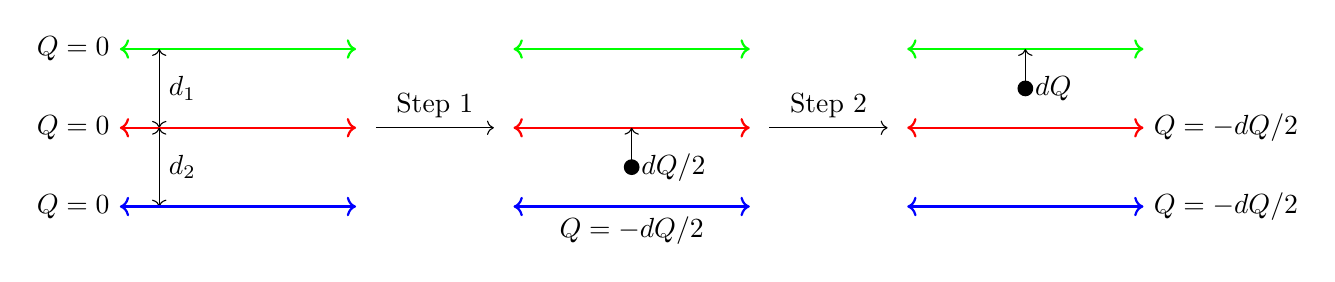
\begin{tikzpicture}
              \draw[<->, green, thick] (0,1)node[black, left]{$Q=0$} -- ++(3,0) ;
              \draw[<->, black] (0.5, 1) -- ++(0,-1) node[midway, right]{$d_1$};
              \draw[<->, red, thick] (0,0) node[black, left]{$Q=0$}-- ++(3,0) ;
              \draw[<->, black] (0.5, 0) -- ++(0,-1) node[midway, right]{$d_2$};
              \draw[<->, blue, thick] (0,-1) node[black,left]{$Q=0$}-- ++(3,0) ;

              \draw[->] (3.25, 0) -- ++(1.5,0) node[midway, above]{Step 1};

              \draw[<->, green, thick] (0+5,1) -- ++(3,0);
              \draw[<->, red, thick] (0+5,0) -- ++(3,0);
              \fill (0+3/2+5,-0.5) circle (0.1) node[right]{$dQ/2$};
              \draw[->] (0+3/2+5,-0.5) -- ++(0,0.5);
              \draw[<->, blue, thick] (0+5,-1) -- ++(3,0) node[black,midway,below]{$Q=-dQ/2$};

              \draw[->] (3.25+5, 0) -- ++(1.5,0) node[midway, above]{Step 2};

              \draw[<->, green, thick] (0+5+5,1) -- ++(3,0);
              \draw[<->, red, thick] (0+5+5,0) -- ++(3,0) node[black,right]{$Q=-dQ/2$};
              \fill (0+3/2+5+5,0.5) circle (0.1) node[right]{$dQ$};
              \draw[->] (0+3/2+5+5,0.5) -- ++(0,0.5);
              \draw[<->, blue, thick] (0+5+5,-1) -- ++(3,0) node[black,right]{$Q=-dQ/2$};
            \end{tikzpicture}
          \end{center}
          Beginning with step 1, we pull our $dQ/2$ off of plate 3 and begin moving it to plate 2.
          This requires work
          $$dW=\bv{F}\cdot\bv{d}=\abs{F}d_2=\abs{QE}d_2=\frac{Qd_2dQ}{4A\epsilon_0}d_2\implies W=\frac{Q^2d_2}{8A\epsilon_0}.$$
          Where we've said that the electric field due to the third plate is
          $$E_3=-\frac{\sigma}{2\epsilon_0}=-\frac{dQ}{4A\epsilon_0}.$$
          Now for the second step we are subject to the previous electric field alongside the electric field created by plate 2
          which is now at charge $-dQ/2$. This means we have a total electric field
          $$E_{23}=-\frac{\sigma}{\epsilon_0}$$
          which gives work
          $$dW=\frac{Qd_1dq}{A\epsilon_0}\implies W=\frac{Q^2d_1}{2A\epsilon_0}.$$
          Summing these to obtain the total work done over the whole process,
          $$W_{tot}=\frac{Q^2d_2}{8A\epsilon_0}+\frac{Q^2d_1}{2A\epsilon_0}=\frac{Q^2}{2A\epsilon_0}\left[d_1+d_2/4\right]$$
    \item Here we use
          $$W=\frac{\epsilon_0}{2}\int \abs{E(\bv{r})}^2\,d^3r.$$
          Our electric field is only defined piecewise due to the discontinuities at the
          plates, so the integral splits up to one smaller integral per region,
          $$
            W=\frac{\epsilon_0}{2}\left[
              \int \abs{E_1(\bv{r})}^2\,d^3r
              +\int \abs{E_2(\bv{r})}^2\,d^3r
              +\int \abs{E_3(\bv{r})}^2\,d^3r
              +\int \abs{E_4(\bv{r})}^2\,d^3r
              \right].
          $$
          Both $E_1$ and $E_4$ are zero as shown in (a) and so those integrals vanish. We are left with
          \begin{align*}
            W & =\frac{\epsilon_0}{2}\left[
              \int \abs{E_2(\bv{r})}^2\,d^3r
              +\int \abs{E_3(\bv{r})}^2\,d^3r
            \right]                                  \\
              & =\frac{\epsilon_0}{2}\left[
              \int_0^{d_1}\int\int \abs{-2\sigma/\epsilon_0}^2\,dxdydz
              +\int_{0}^{d_2}\int\int \abs{-\sigma/\epsilon_0}^2\,dxdydz
            \right]                                  \\
              & =\frac{1}{2\epsilon_0}\left[
              \int_0^{d_1}\int\int 4\sigma^2\,dxdydz
              +\int_{0}^{d_2}\int\int \sigma^2\,dxdydz
            \right]                                  \\
              & =\frac{1}{2\epsilon_0}\left[
              4\sigma^2d_1A
              +\sigma^2d_2A
            \right]                                  \\
              & =\frac{\sigma^2A}{2\epsilon_0}\left[
              4d_1
              +d_2
            \right]                                  \\
              & =\frac{Q^2}{2A\epsilon_0}\left[
              4d_1
              +d_2
              \right]
          \end{align*}
          Which is obviously not the same so I've gone wrong somewhere. Not sure where and I don't have the time to think about it, sorry :(.
  \end{enumerate}
\end{soln}

% PROBLEM 3
\begin{problem}
A uniformly charged solid cylinder has length $L$, radius $R$, and charge density $\rho$.
\begin{enumerate}[label=(\alph*)]
  \item Find the potential on the axis of the cylinder as a function of $z$, the distance along the central axis from
        the centre of the cylinder.
  \item Does the solution to part (a) give you enough information to solve for the electric field along the $z$-axis?
        Why or why not? Hint: Look at the gradient operator in cylindrical coordinates. What assumptions would
        you have to make to calculate $\bv{E}$? Are they reasonable?
\end{enumerate}
\end{problem}
\begin{soln}~
  \begin{enumerate}[label=(\alph*)]
    \item Since we're only interested in the $z$ axis we set $\bv{r}=z\uz$.
          We define $\primed{\bv{r}}=\primed{x}\ux+\primed{y}\uy+\primed{z}\uz$ as usual
          which gives
          $$\bscriptr=-\primed{x}\ux-\primed{y}\uy+\left(z-\primed{z}\right)\uz.$$
          Making the change into cylindrical coordinates with
          \begin{align*}
            \primed{x} & =\primed{s}\cos\primed{\phi} \\
            \primed{y} & =\primed{s}\sin\primed{\phi} \\
            \primed{z} & =\primed{z}
          \end{align*}
          gives us
          $$\bscriptr=-\primed{s}\cos\primed{\phi}\ux-\primed{s}\sin\primed{\phi}\uy+\left(z-\primed{z}\right)\uz.$$
          Now the integral for potential due to volume is
          $$V\left(\bv{r}\right)=\frac{1}{4\pi\epsilon_0}\int \frac{\rho}{\scriptr}d^3\primed{r}$$
          substituting in our $\scriptr$,
          $$V\left(\bv{r}\right)=\frac{1}{4\pi\epsilon_0}\int \frac{\rho}{
              \sqrt{\primed{s}^2\cos^2\primed{\phi}+\primed{s}^2\sin^2\primed{\phi}+\left(z-\primed{z}\right)^2}
            }d^3\primed{r}.$$
          Because we've made the change to cylindrical coordinates the area element $d^3\primed{r}=\primed{s}d\primed{s}d\primed{z}d\primed{\phi}$,
          $$V\left(\bv{r}\right)=\frac{\rho}{4\pi\epsilon_0}\int_0^{2\pi}d\primed{\phi}\int_{-L/2}^{L/2}d\primed{z}\int_0^Rd\primed{s} \frac{\primed{s}}{
              \sqrt{\primed{s}^2\cos^2\primed{\phi}+\primed{s}^2\sin^2\primed{\phi}+\left(z-\primed{z}\right)^2}
            }.$$
          Now evaluating this integral,
          \begin{align*}
            V\left(\bv{r}\right) & =\frac{\rho}{2\epsilon_0}\int_{-L/2}^{L/2}d\primed{z}\int_0^Rd\primed{s} \frac{\primed{s}}{
            \sqrt{\primed{s}^2+\left(z-\primed{z}\right)^2}}                                                                                                                                                     \\
                                 & =\frac{\rho}{4\epsilon_0}\int_{-L/2}^{L/2}d\primed{z}\int_0^Rd\primed{s} \frac{1}{\sqrt{u}}
            \justif{\quad}{$u=\primed{s}^2+\left(z-\primed{z}\right)^2\implies du/2\primed{s}=d\primed{s}$}                                                                                                      \\
                                 & =\frac{\rho}{2\epsilon_0}\int_{-L/2}^{L/2}d\primed{z} \eval{\sqrt{\primed{s}^2+\left(z-\primed{z}\right)^2}}_{0}^{R}                                                          \\
                                 & =\frac{\rho}{2\epsilon_0}\int_{-L/2}^{L/2}d\primed{z} \left[\sqrt{R^2+\left(z-\primed{z}\right)^2}-\abs{z-\primed{z}}\right]                                                  \\
                                 & =\frac{\rho}{2\epsilon_0}\left[\int_{-L/2}^{L/2}\sqrt{R^2+\left(z-\primed{z}\right)^2}d\primed{z}-\int_{-L/2}^{L/2}zd\primed{z}-\int_{-L/2}^{L/2}\primed{z}d\primed{z}\right]
            \justif{\quad}{$z>\primed{z}$ because $\primed{z}\in[-L/2,L/2]$}                                                                                                                                     \\
                                 & =\frac{\rho}{2\epsilon_0}\left[\int_{-L/2}^{L/2}\sqrt{R^2+\left(z-\primed{z}\right)^2}d\primed{z}-zL\right]                                                                   \\
                                 & =\frac{\rho}{2\epsilon_0}\left[\int_{-L/2}^{L/2}\sqrt{R^2+u^2}du-zL\right]\justif{\quad}{$u=\primed{z}-z\implies du=d\primed{z}$}                                             \\
                                 & =\frac{\rho}{2\epsilon_0}\left[\int_{-L/2}^{L/2}R^2\sec^2 v\sqrt{R^2 + R^2\tan^2 v}dv-zL\right]\justif{\quad}{$u=R\tan v\implies du=R\sec^2 v dv$}                            \\
                                 & =\frac{\rho}{2\epsilon_0}\left[\int_{-L/2}^{L/2}R^2\sec^3 v\,dv-zL\right]\justif{\quad}{$R^2\tan^2v +R^2=R^2\sec^2v$}                                                         \\
          \end{align*}
          We could do the integral of $\sec^3$ by parts but I'm just going to use an integral table which gives
          $$\int \sec^3 v \,dv = \frac{1}{2}\left(\sec v \tan v + \ln\abs{\sec v + \tan v}\right)$$
          so,
          \begin{align*}
             & =\frac{\rho}{2\epsilon_0}\left[\frac{R^2}{2}\left(\sec \left(\arctan\left(u/R\right)\right)\tan \left(\arctan\left(u/R\right)\right)\right.\right.                                                                                                   \\
             & \quad \left.\left.+ \eval{\ln\abs{\sec \left(\arctan\left(u/R\right)\right) + \tan \left(\arctan\left(u/R\right)\right)}\right)}_{-L/2}^{L/2}-zL\right]                                                                                              \\
             & =\frac{\rho}{2\epsilon_0}\left[\frac{R^2}{2}\eval{\left(\frac{u}{R}\sqrt{1+u^2/R^2} + \ln\abs{\sqrt{1+u^2/R^2} + u/R}\right)}_{-L/2}^{L/2}-zL\right]                                                                                                 \\
             & =\frac{\rho}{2\epsilon_0}\left[\frac{R^2}{2}\eval{\left(\frac{\left(\primed{z}-z\right)}{R}\sqrt{1+\left(\primed{z}-z\right)^2/R^2} + \ln\abs{\sqrt{1+\left(\primed{z}-z\right)^2/R^2} + \left(\primed{z}-z\right)/R}\right)}_{-L/2}^{L/2}-zL\right] \\
             & =\frac{\rho}{2\epsilon_0}\left[
              \frac{R^2}{2}\left(\frac{\left(L/2-z\right)}{R}\sqrt{1+\left(L/2-z\right)^2/R^2}
            + \ln\abs{\sqrt{1+\left(L/2-z\right)^2/R^2} + \left(L/2-z\right)/R}\right)\right.                                                                                                                                                                       \\
             & \quad\left.-\frac{R^2}{2}\left(\frac{\left(-L/2-z\right)}{R}\sqrt{1+\left(-L/2-z\right)^2/R^2}
              - \ln\abs{\sqrt{1+\left(-L/2-z\right)^2/R^2} + \left(-L/2-z\right)/R}\right)
            -zL\right]                                                                                                                                                                                                                                              \\
          \end{align*}
          Wow! I'm going to use SageMath (a computer algebra system) to simplify that a bit because it's a mess!
          Sage spits out:
          \begin{align*}
             & = \frac{\rho}{\epsilon_0}\left[-2Lz+
              \left(z+L/2\right)\sqrt{R^2+(z+L/2)^2}
            -\left(z-L/2\right)\sqrt{R^2+(z-L/2)^2}\right.                                                                            \\
             & \quad\left.+R^2\ln\left(\frac{\sqrt{R^2+(z+L/2)^2}+\left(z+L/2\right)}{\sqrt{R^2+(z-L/2)^2}+\left(z-L/2\right)}\right)
              \right]
          \end{align*}
    \item Yes, we should be able to find the electric field along $z$ only as we know $V(0,0,z)$. We have to assume, to say we actually know the full field,
    that the field is net zero in $x$ and $y$ which I think should be reasonable because they should cancel eachother out at the axis.
  \end{enumerate}
\end{soln}
\end{document}